%%%%%%%%%%%%%%%%%%%%%%%%%%%%%%%%%%%%%%%%%%%%%%%%%%%%%%%%%%%%%%%%%%%%%%%%%%%%%%%%%%%%%%%%%%%%%%%%
%
% CS484 Written Question Template
%
% Acknowledgements:
% The original code is written by Prof. James Tompkin (james_tompkin@brown.edu).
% The second version is revised by Prof. Min H. Kim (minhkim@kaist.ac.kr).
%
% This is a LaTeX document. LaTeX is a markup language for producing 
% documents. Your task is to fill out this document, then to compile 
% it into a PDF document. 
%
% 
% TO COMPILE:
% > pdflatex thisfile.tex
%
% If you do not have LaTeX and need a LaTeX distribution:
% - Personal laptops (all common OS): www.latex-project.org/get/
% - We recommend latex compiler miktex (https://miktex.org/) for windows,
%   macTex (http://www.tug.org/mactex/) for macOS users.
%   And TeXstudio(http://www.texstudio.org/) for latex editor.
%   You should install both compiler and editor for editing latex.
%   The another option is Overleaf (https://www.overleaf.com/) which is 
%   an online latex editor.
%
% If you need help with LaTeX, please come to office hours. 
% Or, there is plenty of help online:
% https://en.wikibooks.org/wiki/LaTeX
%
% Good luck!
% Min and the CS484 staff
%
%%%%%%%%%%%%%%%%%%%%%%%%%%%%%%%%%%%%%%%%%%%%%%%%%%%%%%%%%%%%%%%%%%%%%%%%%%%%%%%%%%%%%%%%%%%%%%%%
%
% How to include two graphics on the same line:
% 
% \includegraphics[width=0.49\linewidth]{yourgraphic1.png}
% \includegraphics[width=0.49\linewidth]{yourgraphic2.png}
%
% How to include equations:
%
% \begin{equation}
% y = mx+c
% \end{equation}
% 
%%%%%%%%%%%%%%%%%%%%%%%%%%%%%%%%%%%%%%%%%%%%%%%%%%%%%%%%%%%%%%%%%%%%%%%%%%%%%%%%%%%%%%%%%%%%%%%%

\documentclass[11pt]{article}

\usepackage[english]{babel}
\usepackage[utf8]{inputenc}
\usepackage[colorlinks = true,
linkcolor = blue,
urlcolor  = blue]{hyperref}
\usepackage[a4paper,margin=1.5in]{geometry}
\usepackage{stackengine,graphicx}
\usepackage{fancyhdr}
\setlength{\headheight}{15pt}
\usepackage{microtype}
\usepackage{times}

% From https://ctan.org/pkg/matlab-prettifier
\usepackage[numbered,framed]{matlab-prettifier}

\frenchspacing
\setlength{\parindent}{0cm} % Default is 15pt.
\setlength{\parskip}{0.3cm plus1mm minus1mm}

\pagestyle{fancy}
\fancyhf{}
\lhead{Homework 2 Questions}
\rhead{CS484}
\rfoot{\thepage}

\date{}

\title{\vspace{-1cm}Homework 2 Questions}

\begin{document}
	\maketitle
	\vspace{-3cm}
	\thispagestyle{fancy}
	
	\section*{Instructions}
	\begin{itemize}
		\item 4 questions.
		\item Write code where appropriate.
		\item Feel free to include images or equations.
		\item \textbf{Please use only the space provided and keep the page breaks.} Please do not make new pages, nor remove pages. The document is a template to help grading.
		\item If you really need extra space, please use new pages at the end of the document and refer us to it in your answers.
	\end{itemize}

	\section*{Questions}
	
	\paragraph{Q1:} Explicitly describe image convolution: the input, the transformation, and the output. Why is it useful for computer vision?
	
	%%%%%%%%%%%%%%%%%%%%%%%%%%%%%%%%%%%
	\paragraph{A1:} 
	 Convolution is a process of transforming the image by adding elements of given image to its neighbors which is weighted by the filter or kernel, using the form of mathematical convolution. 
	 
	 With the input of image pieces and given kernel, this process changes image pieces using filters, calculating the convolution of matrices, which returns new sealed image matrix. 
	 
	 Image convolution is widely used in various parts on computer vision, including blurring or image processing.
	
	
	
	%%%%%%%%%%%%%%%%%%%%%%%%%%%%%%%%%%%
	
	% Please leave the pagebreak
	\pagebreak
	\paragraph{Q2:} What is the difference between convolution and correlation? Construct a scenario which produces a different output between both operations.
	
	\emph{Please use \href{https://www.mathworks.com/help/images/ref/imfilter.html}{$imfilter$} to experiment! Look at the `options' parameter in MATLAB Help to learn how to switch the underlying operation from correlation to convolution.}
	
	%%%%%%%%%%%%%%%%%%%%%%%%%%%%%%%%%%%
	\paragraph{A2:} Theoretically, convolution are linear operations on the signal or signal modifiers, whereas correlation is a measure of similarity between two signals. The basic difference is that convolution rotates the matrix by 180 degrees. 
	
	With the code written below, we can easily check out the difference of two different methods, which convoluted figure is flipped compared to correlated figure.
	
	\begin{lstlisting}[style=Matlab-editor]
function problem2()

    image = im2single(imread('../data/cat.bmp'));
    filter =  [-0.5 0 0.5; -1 0 1; -0.5 0 0.5];
    
    imgcorr = imfilter(image, filter, "corr");
    imgconv = imfilter(image, filter, 'conv');
    
    figure(1) ; imshow(imgcorr);
    figure(2) ; imshow(imgconv);

end
\end{lstlisting}
	
	
	
	%%%%%%%%%%%%%%%%%%%%%%%%%%%%%%%%%%%
	
	% Please leave the pagebreak
	\pagebreak
	\paragraph{Q3:} What is the difference between a high pass filter and a low pass filter in how they are constructed, and what they do to the image? Please provide example kernels and output images.
	
	%%%%%%%%%%%%%%%%%%%%%%%%%%%%%%%%%%%
	\paragraph{A3:} Low pass filters, which are usually used on blurring filters, denotes smooth regions. All the values in low pass filters are positive, which edge content is reduced by them. As the size of the filter grows, the more smoothing effect will take place. 
	
	High pass filters, in contrast, both have positive and as well as negative values and increases edge contents. This results that if the size of the mask grows, more edge content is increased.
	
	A typical low and high pass filter can be given as below
	
\begin{lstlisting}[style=Matlab-editor]
function problem2()

    image = im2single(imread('../data/cat.bmp'));
    low_filter =  [0,0,0,0,0; 0,0,0,0,0; 0,0,1,0,0; 0,0,0,0,0; 0,0,0,0,0];
    high_filter = 1/24*[1,1,1,1,1; 1,1,1,1,1; 1,1,0,1,1; 1,1,1,1,1; 1,1,1,1,1]
    
    imgLow = imfilter(image, low_filter);
    imgHigh = imfilter(image, high_filter);
    
    figure(1) ; imshow(imgLow);
    figure(2) ; imshow(imgHigh);

end
\end{lstlisting}	
	
	As the result of each figures, figure 1 and 2 is given below (Left is figure 1, right is figure 2)
	
	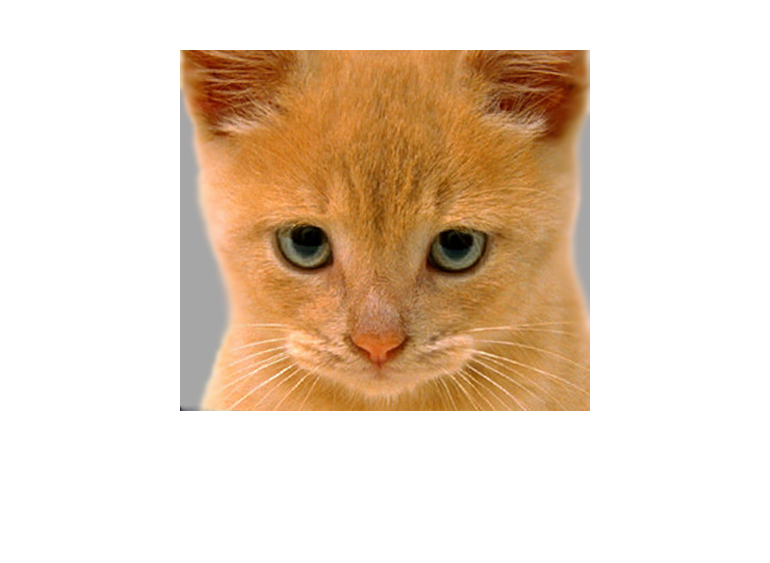
\includegraphics[scale=0.35]{fig1}  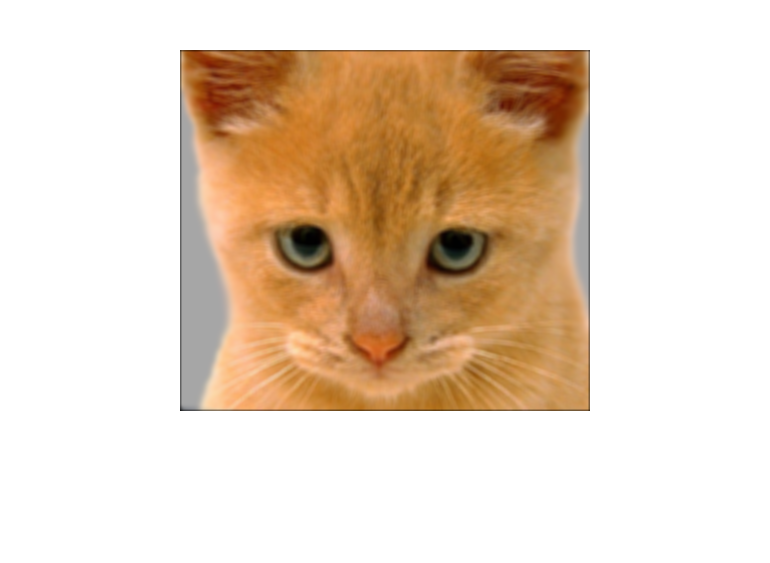
\includegraphics[scale=0.35]{fig2}
	


	
	
	
	%%%%%%%%%%%%%%%%%%%%%%%%%%%%%%%%%%%
	
	% Please leave the pagebreak
	\pagebreak
	\paragraph{Q4:} How does computation time vary with filter sizes from $3\times3$ to $15\times15$ (for all odd and square sizes), and with image sizes from 0.25~MPix to 8~MPix (choose your own intervals)? Measure both using \href{https://www.mathworks.com/help/images/ref/imfilter.html}{$imfilter$} to produce a matrix of values. Use the \href{https://www.mathworks.com/help/images/ref/imresize.html}{$imresize$} function to vary the size of an image. Use an appropriate charting function to plot your matrix of results, such as \href{https://www.mathworks.com/help/matlab/ref/scatter3.html}{$scatter3$} or \href{https://www.mathworks.com/help/matlab/ref/surf.html}{$surf$}.
	
	Do the results match your expectation given the number of multiply and add operations in convolution?
	
	See RISDance.jpg in the attached file.
	
	%%%%%%%%%%%%%%%%%%%%%%%%%%%%%%%%%%%
	\paragraph{A4:} 
	\begin{lstlisting}[style=Matlab-editor]
	function question4()
    %QUESTION4 이 함수의 요약 설명 위치
    %   자세한 설명 위치
        [X,Y] = meshgrid(1:7,1:32);
        Z = func1(X,Y);
        surf(X,Y,Z);
    end

    function result =  func1(i, j) 
        image = imread('./RISDance.jpg');
        k = 0.08*j;
        image_j = imresize(image, k);
        filter = zeros(2*i+1);
        filter(i+1,i+1) = 1;
        tic
        new_img=imfilter(image_j, filter);
        elapsedTime = toc;
        result = single(elapsedTime);
       
    end
	\end{lstlisting}
	
	As using the code written above, I could check the time variance when we vary the size the size of the image and the filter.
	
	It increased severely while I increase the size of the image, and insignificantly while I increased the size of the filter.
	
	%%%%%%%%%%%%%%%%%%%%%%%%%%%%%%%%%%%
	
	
	% If you really need extra space, uncomment here and use extra pages after the last question.
	% Please refer here in your original answer. Thanks!
	%\pagebreak
	%\paragraph{AX.X Continued:} Your answer continued here.
	
	
	
\end{document}